
% Default to the notebook output style

    


% Inherit from the specified cell style.




    
\documentclass{article}

    
    \usepackage{float}
    \usepackage{graphicx} % Used to insert images
    \usepackage{adjustbox} % Used to constrain images to a maximum size 
    \usepackage{color} % Allow colors to be defined
    \usepackage{enumerate} % Needed for markdown enumerations to work
    \usepackage{geometry} % Used to adjust the document margins
    \usepackage{amsmath} % Equations
    \usepackage{amssymb} % Equations
    \usepackage{eurosym} % defines \euro
    \usepackage[mathletters]{ucs} % Extended unicode (utf-8) support
    \usepackage[utf8x]{inputenc} % Allow utf-8 characters in the tex document
    \usepackage{fancyvrb} % verbatim replacement that allows latex
    \usepackage{grffile} % extends the file name processing of package graphics 
                         % to support a larger range 
    % The hyperref package gives us a pdf with properly built
    % internal navigation ('pdf bookmarks' for the table of contents,
    % internal cross-reference links, web links for URLs, etc.)
    \usepackage{hyperref}
    \usepackage{longtable} % longtable support required by pandoc >1.10
    \usepackage{booktabs}  % table support for pandoc > 1.12.2
    \usepackage{ulem} % ulem is needed to support strikethroughs (\sout)
    

    
    
    \definecolor{orange}{cmyk}{0,0.4,0.8,0.2}
    \definecolor{darkorange}{rgb}{.71,0.21,0.01}
    \definecolor{darkgreen}{rgb}{.12,.54,.11}
    \definecolor{myteal}{rgb}{.26, .44, .56}
    \definecolor{gray}{gray}{0.45}
    \definecolor{lightgray}{gray}{.95}
    \definecolor{mediumgray}{gray}{.8}
    \definecolor{inputbackground}{rgb}{.95, .95, .85}
    \definecolor{outputbackground}{rgb}{.95, .95, .95}
    \definecolor{traceback}{rgb}{1, .95, .95}
    % ansi colors
    \definecolor{red}{rgb}{.6,0,0}
    \definecolor{green}{rgb}{0,.65,0}
    \definecolor{brown}{rgb}{0.6,0.6,0}
    \definecolor{blue}{rgb}{0,.145,.698}
    \definecolor{purple}{rgb}{.698,.145,.698}
    \definecolor{cyan}{rgb}{0,.698,.698}
    \definecolor{lightgray}{gray}{0.5}
    
    % bright ansi colors
    \definecolor{darkgray}{gray}{0.25}
    \definecolor{lightred}{rgb}{1.0,0.39,0.28}
    \definecolor{lightgreen}{rgb}{0.48,0.99,0.0}
    \definecolor{lightblue}{rgb}{0.53,0.81,0.92}
    \definecolor{lightpurple}{rgb}{0.87,0.63,0.87}
    \definecolor{lightcyan}{rgb}{0.5,1.0,0.83}
    
    % commands and environments needed by pandoc snippets
    % extracted from the output of `pandoc -s`
    \providecommand{\tightlist}{%
      \setlength{\itemsep}{0pt}\setlength{\parskip}{0pt}}
    \DefineVerbatimEnvironment{Highlighting}{Verbatim}{commandchars=\\\{\}}
    % Add ',fontsize=\small' for more characters per line
    \newenvironment{Shaded}{}{}
    \newcommand{\KeywordTok}[1]{\textcolor[rgb]{0.00,0.44,0.13}{\textbf{{#1}}}}
    \newcommand{\DataTypeTok}[1]{\textcolor[rgb]{0.56,0.13,0.00}{{#1}}}
    \newcommand{\DecValTok}[1]{\textcolor[rgb]{0.25,0.63,0.44}{{#1}}}
    \newcommand{\BaseNTok}[1]{\textcolor[rgb]{0.25,0.63,0.44}{{#1}}}
    \newcommand{\FloatTok}[1]{\textcolor[rgb]{0.25,0.63,0.44}{{#1}}}
    \newcommand{\CharTok}[1]{\textcolor[rgb]{0.25,0.44,0.63}{{#1}}}
    \newcommand{\StringTok}[1]{\textcolor[rgb]{0.25,0.44,0.63}{{#1}}}
    \newcommand{\CommentTok}[1]{\textcolor[rgb]{0.38,0.63,0.69}{\textit{{#1}}}}
    \newcommand{\OtherTok}[1]{\textcolor[rgb]{0.00,0.44,0.13}{{#1}}}
    \newcommand{\AlertTok}[1]{\textcolor[rgb]{1.00,0.00,0.00}{\textbf{{#1}}}}
    \newcommand{\FunctionTok}[1]{\textcolor[rgb]{0.02,0.16,0.49}{{#1}}}
    \newcommand{\RegionMarkerTok}[1]{{#1}}
    \newcommand{\ErrorTok}[1]{\textcolor[rgb]{1.00,0.00,0.00}{\textbf{{#1}}}}
    \newcommand{\NormalTok}[1]{{#1}}
    
    % Additional commands for more recent versions of Pandoc
    \newcommand{\ConstantTok}[1]{\textcolor[rgb]{0.53,0.00,0.00}{{#1}}}
    \newcommand{\SpecialCharTok}[1]{\textcolor[rgb]{0.25,0.44,0.63}{{#1}}}
    \newcommand{\VerbatimStringTok}[1]{\textcolor[rgb]{0.25,0.44,0.63}{{#1}}}
    \newcommand{\SpecialStringTok}[1]{\textcolor[rgb]{0.73,0.40,0.53}{{#1}}}
    \newcommand{\ImportTok}[1]{{#1}}
    \newcommand{\DocumentationTok}[1]{\textcolor[rgb]{0.73,0.13,0.13}{\textit{{#1}}}}
    \newcommand{\AnnotationTok}[1]{\textcolor[rgb]{0.38,0.63,0.69}{\textbf{\textit{{#1}}}}}
    \newcommand{\CommentVarTok}[1]{\textcolor[rgb]{0.38,0.63,0.69}{\textbf{\textit{{#1}}}}}
    \newcommand{\VariableTok}[1]{\textcolor[rgb]{0.10,0.09,0.49}{{#1}}}
    \newcommand{\ControlFlowTok}[1]{\textcolor[rgb]{0.00,0.44,0.13}{\textbf{{#1}}}}
    \newcommand{\OperatorTok}[1]{\textcolor[rgb]{0.40,0.40,0.40}{{#1}}}
    \newcommand{\BuiltInTok}[1]{{#1}}
    \newcommand{\ExtensionTok}[1]{{#1}}
    \newcommand{\PreprocessorTok}[1]{\textcolor[rgb]{0.74,0.48,0.00}{{#1}}}
    \newcommand{\AttributeTok}[1]{\textcolor[rgb]{0.49,0.56,0.16}{{#1}}}
    \newcommand{\InformationTok}[1]{\textcolor[rgb]{0.38,0.63,0.69}{\textbf{\textit{{#1}}}}}
    \newcommand{\WarningTok}[1]{\textcolor[rgb]{0.38,0.63,0.69}{\textbf{\textit{{#1}}}}}
    
    
    % Define a nice break command that doesn't care if a line doesn't already
    % exist.
    \def\br{\hspace*{\fill} \\* }
    % Math Jax compatability definitions
    \def\gt{>}
    \def\lt{<}
    % Document parameters
    \title{Review of Statistical Analysis of Numerical Preclinical Radio-biological Data}
    \author{Raaz Dwivedi$^+$,  Antonio Iannopollo$^+$ and Jiancong Chen$^*$ \\
    $^+$Department of EECS, $^*$Department of Civil \& Environmental Engineering \\
    University of California, Berkeley}
    
    
    

    % Pygments definitions
    
\makeatletter
\def\PY@reset{\let\PY@it=\relax \let\PY@bf=\relax%
    \let\PY@ul=\relax \let\PY@tc=\relax%
    \let\PY@bc=\relax \let\PY@ff=\relax}
\def\PY@tok#1{\csname PY@tok@#1\endcsname}
\def\PY@toks#1+{\ifx\relax#1\empty\else%
    \PY@tok{#1}\expandafter\PY@toks\fi}
\def\PY@do#1{\PY@bc{\PY@tc{\PY@ul{%
    \PY@it{\PY@bf{\PY@ff{#1}}}}}}}
\def\PY#1#2{\PY@reset\PY@toks#1+\relax+\PY@do{#2}}

\expandafter\def\csname PY@tok@gd\endcsname{\def\PY@tc##1{\textcolor[rgb]{0.63,0.00,0.00}{##1}}}
\expandafter\def\csname PY@tok@gu\endcsname{\let\PY@bf=\textbf\def\PY@tc##1{\textcolor[rgb]{0.50,0.00,0.50}{##1}}}
\expandafter\def\csname PY@tok@gt\endcsname{\def\PY@tc##1{\textcolor[rgb]{0.00,0.27,0.87}{##1}}}
\expandafter\def\csname PY@tok@gs\endcsname{\let\PY@bf=\textbf}
\expandafter\def\csname PY@tok@gr\endcsname{\def\PY@tc##1{\textcolor[rgb]{1.00,0.00,0.00}{##1}}}
\expandafter\def\csname PY@tok@cm\endcsname{\let\PY@it=\textit\def\PY@tc##1{\textcolor[rgb]{0.25,0.50,0.50}{##1}}}
\expandafter\def\csname PY@tok@vg\endcsname{\def\PY@tc##1{\textcolor[rgb]{0.10,0.09,0.49}{##1}}}
\expandafter\def\csname PY@tok@vi\endcsname{\def\PY@tc##1{\textcolor[rgb]{0.10,0.09,0.49}{##1}}}
\expandafter\def\csname PY@tok@mh\endcsname{\def\PY@tc##1{\textcolor[rgb]{0.40,0.40,0.40}{##1}}}
\expandafter\def\csname PY@tok@cs\endcsname{\let\PY@it=\textit\def\PY@tc##1{\textcolor[rgb]{0.25,0.50,0.50}{##1}}}
\expandafter\def\csname PY@tok@ge\endcsname{\let\PY@it=\textit}
\expandafter\def\csname PY@tok@vc\endcsname{\def\PY@tc##1{\textcolor[rgb]{0.10,0.09,0.49}{##1}}}
\expandafter\def\csname PY@tok@il\endcsname{\def\PY@tc##1{\textcolor[rgb]{0.40,0.40,0.40}{##1}}}
\expandafter\def\csname PY@tok@go\endcsname{\def\PY@tc##1{\textcolor[rgb]{0.53,0.53,0.53}{##1}}}
\expandafter\def\csname PY@tok@cp\endcsname{\def\PY@tc##1{\textcolor[rgb]{0.74,0.48,0.00}{##1}}}
\expandafter\def\csname PY@tok@gi\endcsname{\def\PY@tc##1{\textcolor[rgb]{0.00,0.63,0.00}{##1}}}
\expandafter\def\csname PY@tok@gh\endcsname{\let\PY@bf=\textbf\def\PY@tc##1{\textcolor[rgb]{0.00,0.00,0.50}{##1}}}
\expandafter\def\csname PY@tok@ni\endcsname{\let\PY@bf=\textbf\def\PY@tc##1{\textcolor[rgb]{0.60,0.60,0.60}{##1}}}
\expandafter\def\csname PY@tok@nl\endcsname{\def\PY@tc##1{\textcolor[rgb]{0.63,0.63,0.00}{##1}}}
\expandafter\def\csname PY@tok@nn\endcsname{\let\PY@bf=\textbf\def\PY@tc##1{\textcolor[rgb]{0.00,0.00,1.00}{##1}}}
\expandafter\def\csname PY@tok@no\endcsname{\def\PY@tc##1{\textcolor[rgb]{0.53,0.00,0.00}{##1}}}
\expandafter\def\csname PY@tok@na\endcsname{\def\PY@tc##1{\textcolor[rgb]{0.49,0.56,0.16}{##1}}}
\expandafter\def\csname PY@tok@nb\endcsname{\def\PY@tc##1{\textcolor[rgb]{0.00,0.50,0.00}{##1}}}
\expandafter\def\csname PY@tok@nc\endcsname{\let\PY@bf=\textbf\def\PY@tc##1{\textcolor[rgb]{0.00,0.00,1.00}{##1}}}
\expandafter\def\csname PY@tok@nd\endcsname{\def\PY@tc##1{\textcolor[rgb]{0.67,0.13,1.00}{##1}}}
\expandafter\def\csname PY@tok@ne\endcsname{\let\PY@bf=\textbf\def\PY@tc##1{\textcolor[rgb]{0.82,0.25,0.23}{##1}}}
\expandafter\def\csname PY@tok@nf\endcsname{\def\PY@tc##1{\textcolor[rgb]{0.00,0.00,1.00}{##1}}}
\expandafter\def\csname PY@tok@si\endcsname{\let\PY@bf=\textbf\def\PY@tc##1{\textcolor[rgb]{0.73,0.40,0.53}{##1}}}
\expandafter\def\csname PY@tok@s2\endcsname{\def\PY@tc##1{\textcolor[rgb]{0.73,0.13,0.13}{##1}}}
\expandafter\def\csname PY@tok@nt\endcsname{\let\PY@bf=\textbf\def\PY@tc##1{\textcolor[rgb]{0.00,0.50,0.00}{##1}}}
\expandafter\def\csname PY@tok@nv\endcsname{\def\PY@tc##1{\textcolor[rgb]{0.10,0.09,0.49}{##1}}}
\expandafter\def\csname PY@tok@s1\endcsname{\def\PY@tc##1{\textcolor[rgb]{0.73,0.13,0.13}{##1}}}
\expandafter\def\csname PY@tok@ch\endcsname{\let\PY@it=\textit\def\PY@tc##1{\textcolor[rgb]{0.25,0.50,0.50}{##1}}}
\expandafter\def\csname PY@tok@m\endcsname{\def\PY@tc##1{\textcolor[rgb]{0.40,0.40,0.40}{##1}}}
\expandafter\def\csname PY@tok@gp\endcsname{\let\PY@bf=\textbf\def\PY@tc##1{\textcolor[rgb]{0.00,0.00,0.50}{##1}}}
\expandafter\def\csname PY@tok@sh\endcsname{\def\PY@tc##1{\textcolor[rgb]{0.73,0.13,0.13}{##1}}}
\expandafter\def\csname PY@tok@ow\endcsname{\let\PY@bf=\textbf\def\PY@tc##1{\textcolor[rgb]{0.67,0.13,1.00}{##1}}}
\expandafter\def\csname PY@tok@sx\endcsname{\def\PY@tc##1{\textcolor[rgb]{0.00,0.50,0.00}{##1}}}
\expandafter\def\csname PY@tok@bp\endcsname{\def\PY@tc##1{\textcolor[rgb]{0.00,0.50,0.00}{##1}}}
\expandafter\def\csname PY@tok@c1\endcsname{\let\PY@it=\textit\def\PY@tc##1{\textcolor[rgb]{0.25,0.50,0.50}{##1}}}
\expandafter\def\csname PY@tok@o\endcsname{\def\PY@tc##1{\textcolor[rgb]{0.40,0.40,0.40}{##1}}}
\expandafter\def\csname PY@tok@kc\endcsname{\let\PY@bf=\textbf\def\PY@tc##1{\textcolor[rgb]{0.00,0.50,0.00}{##1}}}
\expandafter\def\csname PY@tok@c\endcsname{\let\PY@it=\textit\def\PY@tc##1{\textcolor[rgb]{0.25,0.50,0.50}{##1}}}
\expandafter\def\csname PY@tok@mf\endcsname{\def\PY@tc##1{\textcolor[rgb]{0.40,0.40,0.40}{##1}}}
\expandafter\def\csname PY@tok@err\endcsname{\def\PY@bc##1{\setlength{\fboxsep}{0pt}\fcolorbox[rgb]{1.00,0.00,0.00}{1,1,1}{\strut ##1}}}
\expandafter\def\csname PY@tok@mb\endcsname{\def\PY@tc##1{\textcolor[rgb]{0.40,0.40,0.40}{##1}}}
\expandafter\def\csname PY@tok@ss\endcsname{\def\PY@tc##1{\textcolor[rgb]{0.10,0.09,0.49}{##1}}}
\expandafter\def\csname PY@tok@sr\endcsname{\def\PY@tc##1{\textcolor[rgb]{0.73,0.40,0.53}{##1}}}
\expandafter\def\csname PY@tok@mo\endcsname{\def\PY@tc##1{\textcolor[rgb]{0.40,0.40,0.40}{##1}}}
\expandafter\def\csname PY@tok@kd\endcsname{\let\PY@bf=\textbf\def\PY@tc##1{\textcolor[rgb]{0.00,0.50,0.00}{##1}}}
\expandafter\def\csname PY@tok@mi\endcsname{\def\PY@tc##1{\textcolor[rgb]{0.40,0.40,0.40}{##1}}}
\expandafter\def\csname PY@tok@kn\endcsname{\let\PY@bf=\textbf\def\PY@tc##1{\textcolor[rgb]{0.00,0.50,0.00}{##1}}}
\expandafter\def\csname PY@tok@cpf\endcsname{\let\PY@it=\textit\def\PY@tc##1{\textcolor[rgb]{0.25,0.50,0.50}{##1}}}
\expandafter\def\csname PY@tok@kr\endcsname{\let\PY@bf=\textbf\def\PY@tc##1{\textcolor[rgb]{0.00,0.50,0.00}{##1}}}
\expandafter\def\csname PY@tok@s\endcsname{\def\PY@tc##1{\textcolor[rgb]{0.73,0.13,0.13}{##1}}}
\expandafter\def\csname PY@tok@kp\endcsname{\def\PY@tc##1{\textcolor[rgb]{0.00,0.50,0.00}{##1}}}
\expandafter\def\csname PY@tok@w\endcsname{\def\PY@tc##1{\textcolor[rgb]{0.73,0.73,0.73}{##1}}}
\expandafter\def\csname PY@tok@kt\endcsname{\def\PY@tc##1{\textcolor[rgb]{0.69,0.00,0.25}{##1}}}
\expandafter\def\csname PY@tok@sc\endcsname{\def\PY@tc##1{\textcolor[rgb]{0.73,0.13,0.13}{##1}}}
\expandafter\def\csname PY@tok@sb\endcsname{\def\PY@tc##1{\textcolor[rgb]{0.73,0.13,0.13}{##1}}}
\expandafter\def\csname PY@tok@k\endcsname{\let\PY@bf=\textbf\def\PY@tc##1{\textcolor[rgb]{0.00,0.50,0.00}{##1}}}
\expandafter\def\csname PY@tok@se\endcsname{\let\PY@bf=\textbf\def\PY@tc##1{\textcolor[rgb]{0.73,0.40,0.13}{##1}}}
\expandafter\def\csname PY@tok@sd\endcsname{\let\PY@it=\textit\def\PY@tc##1{\textcolor[rgb]{0.73,0.13,0.13}{##1}}}

\def\PYZbs{\char`\\}
\def\PYZus{\char`\_}
\def\PYZob{\char`\{}
\def\PYZcb{\char`\}}
\def\PYZca{\char`\^}
\def\PYZam{\char`\&}
\def\PYZlt{\char`\<}
\def\PYZgt{\char`\>}
\def\PYZsh{\char`\#}
\def\PYZpc{\char`\%}
\def\PYZdl{\char`\$}
\def\PYZhy{\char`\-}
\def\PYZsq{\char`\'}
\def\PYZdq{\char`\"}
\def\PYZti{\char`\~}
% for compatibility with earlier versions
\def\PYZat{@}
\def\PYZlb{[}
\def\PYZrb{]}
\makeatother


    % Exact colors from NB
    \definecolor{incolor}{rgb}{0.0, 0.0, 0.5}
    \definecolor{outcolor}{rgb}{0.545, 0.0, 0.0}




    % Prevent overflowing lines due to hard-to-break entities
    \sloppy
    % Setup hyperref package
    \hypersetup{
      breaklinks=true,  % so long urls are correctly broken across lines
      colorlinks=true,
      urlcolor=blue,
      linkcolor=black,
      citecolor=darkgreen,
      }
    % Slightly bigger margins than the latex defaults

    \geometry{verbose,tmargin=1in,bmargin=1in,lmargin=1in,rmargin=1in}



    \begin{document}


    \maketitle



\begin{abstract}
This review reproduces tests and results
presented by Pitt and Hill and discusses some other non-parametric techniques, such as Permutation Tests, which allow to analyze data with less restrictive assumptions.
The focus of the review is on the statistical methodology rather than the underlying biological aspects and assumptions of the original work, which are not discussed.
Although not expert in statistical methods for fraud detection, we do believe that permutation tests are promising in this context, as demonstrated by the results presented here.
This review has been developed as a term
project for a Graduate Level Course on Statistical Models at UC Berkeley.
\end{abstract}

\section{Introduction} % (fold)
\label{sec:introduction}

% section introduction (end)

We review the paper in the spirit of promoting reproducibility of research and attempt to replicate the authors' work. We also discuss other methods to identify anomalies, and present results based on our analysis using Permutation Tests. 
Permutation tests are consistent with the aim of the paper--providing simple tools to detect anomalies--and validate the results in the paper, leading to the same conclusions.

Before diving into technical details, we make a minor observation: the organization of the paper was not properly introduced. The use of distinct sections for (1) the discussion on data and experiments; (2) their model and related calculations; (3) the application of common tests from the literature; and (4) conclusions, would have been helpful. The review is organized as follows. In section~\ref{reproducibility-of-results} we replicate authors' work and results and discuss weaknesses of their approach.
In section~\ref{our-analysis}, we propose and implement additional tests to consolidate the results.
We finally draw our conclusions in section~\ref{conclusion}.


\subsection{Problem Set Up}\label{problem-set-up}

The paper begins by voicing a growing concern towards ``Scientific fraud
and Plagiarism'' in the scientific community and is successful in
conveying a strong message.
The authors present some statistical figures and point out the existence of easy statistical tools to detect fabricated data and ignorance about such tools.

The authors examine datsets from radio-biological experiments. They find that data reported by one of 10 researchers, the ``RTS'', is suspicious.
They perform three different tests to validate their suspicion and also validate their tests and assumptions by looking at the data obtained from three other sources.
Each researcher made two types of triple measurements - colony counts and Coulter counts.
The authors suspect that the RTS fabricated data triples to get the mean s/he desired in each triple by setting one observation equal to the desired mean and the other two roughly equidistant above and below that value.
This would result in triples that contain the (rounded) mean as one of their values.

The methodological contribution of the paper is “bounds and estimates for the probability that a given set of $n$ such triples contains $k$ or more triples which contain their own mean” when each of the $n$ triples is independent and identically distributed (i.i.d.) Poisson, and triples are independent of each other.
(Different triples may have different Poisson means.)
For this Poisson model, the chance that the RTS's data would contain so many triples that include their rounded mean is astronomically low.
They also apply more common tests for anomalous data, based on statistics such as the frequency of the terminal digit and the frequency with which the last two digits are equal.
However, some of the questions that were slightly untouched upon are discussed below:

\begin{itemize}
\item
  The authors write, “Having observed what appeared to us to be an unusual frequency of triples in RTS's data containing a value close to their mean, we used R to calculate the mid-ratios for all of the colony data triples that were available to us.” This suggests that the same data--and the same feature of the data--that raised their suspicions about the RTS was the data used to test whether the RTS's data were anomalous on the basis of that feature. If so, then the nominal $p$-values are likely to be misleadingly small.

\item
  Most of the tests assume a model for the observations and compare the RTS's data to that model.
  The authors validate the assumptions of the model by comparing it with the data pooled for the other researchers.
  Pooling the data in this way may hide anomalies in the other researchers' data.
  Permutation tests allow the data from each researcher to be compared to the data from the other researchers without positing a generative model for the data.
  On the other hand, the bulk of the data available is from the RTS.
  To reject the hypothesis that another researcher's data looks like a random sample from the pooled data, if it includes the RTS's data, does not imply s/he is suspicious.
  Instead, it shows that his/her data is not like that of the RTS.
  See section~\ref{our-analysis} of this review for more discussion.
\end{itemize}

    \section{Reproducibility of Results}\label{reproducibility-of-results}

This section discusses our efforts to replicate the analyses in the paper.
After fine tuning, we were able to replicate most of
their results, obtaining similar results in the other cases.
Our work is available on \hyperlink{https://github.com/ianno/stat215a_project1}{github} [github.com/ianno/stat215a\_project1]. We first discuss specifics about the replication and then comment about the tests and methods involved.


    \subsection{Mid-Ratio Analysis}\label{mid-ratio-analysis}

The authors first consider the mid-ratio, which is defined for a triple \((a, b, c), a<b<c\) as
\(\frac{b-a}{c-a}\), and show that the histogram of RTS's data concentrates
abnormally around the \(0.4-0.6\) range, compared to the data taken by all the other lab members.
After tweaking the default histogram function on numpy, we were able to obtain plots similar to the ones reported in Figure (1) of the paper. Two noticeable differences were - (1) we obtain $44\%$ chance of seeing mid-ratio in $(0.4, 0.5]$ interval for RTS, compared to $50\%$ chance reported in the paper and (2) we used 1360/1361 and 595/595 triples to compute histogram for RTS and the rest respectively, compared to the use of 1343/1361 and 572/595 triples by the authors.
We believe the authors did not provide enough information about the methods used to filter data for this section. However, such minor differences did not demand further investigation.

    \subsection{Probability Model and Hypothesis Tests}\label{probability-model}

The authors develop a model to bound the probability of observing $k$ out of $n$ triples contain their mean.
Each entry in a triple is assumed to be an independent sample from a Poisson distribution with mean $\lambda$. (Different triples may have different means.)
The event of observing the rounded mean in such a triple is a Bernoulli random variable (BRV) whose success probability depends on $\lambda$.
The authors derive analytical expressions for these success probabilities in Appendix A.
Numerical values of these probabilities, for $\lambda=\{1, \ldots, 25\}$, are presented in Table 1.
We could replicate this table exactly.
For large $\lambda\ (>2000)$, for which the authors provide only few representative probability values, our implementation suffered from numerical issues.

Using Table 1, the authors determine the success probability for the BRV in two different ways and use it to compute the chance of observing the data.  For hypothesis test I (non-parametric) they used the maximum value from Table 1 as an upper bound for all triples, essentially treating all BRVs as i.i.d. Bernoulli($0.42$). Replicating this was straightforward.
For hypothesis test II and III, the authors use maximum likelihood estimate of $\lambda$ for each triple to compute the corresponding success probability values, essentially treating each BRV to have a different distribution. The authors address the sum of these BRVs as a ``Poisson Binomial Random Variable".
Additionally, for the hypothesis test III, the authors use normal approximation for the Poisson binomial random variables. 
We could replicate the probability values, up to minor errors, for the colony data. 
Limitations of our implementation gave inaccurate results for Coulter data. 
For sanity checks of the results, we used linearly interpolated estimates from the paper (for intermediate $\lambda$) and obtained values similar to those in the paper for these tests. Figure~\ref{table2} is the approximate replication of Table 2 from the paper.

\begin{figure}[H]
\centering
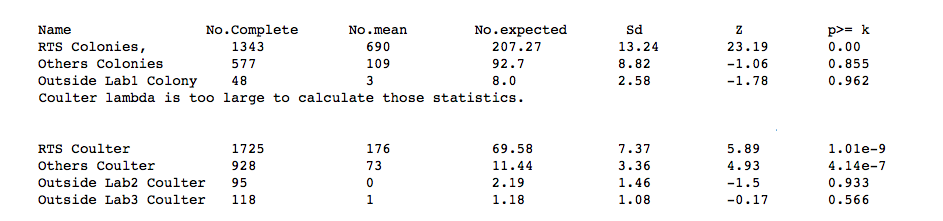
\includegraphics[width=0.9\linewidth]{images/HT_Stat_values.png}
\caption{Approximate Replication of Table 2}
\label{table2}
\end{figure}

    \subsection{Digits Analysis}\label{digits-analysis}

The authors also perform some common tests for fraud detection - \textit{terminal
digit analysis} and \textit{pair of equal terminal digits analysis}. These tests
are based on the assumption that, in general, insignificant digits of a random sample are uniformly distributed.

\subsubsection{Terminal Digit Analysis}\label{terminal-digit-analysis}

The first test assumes that the last digit in samples of large numbers
($>100$) should empirically show uniform distribution. 
Also, some previous works, e.g. \cite{mosimann2002terminal},
have shown that fabricated data often fails to show such peculiar property.
The authors use the chi-square test for goodness of fit, and get low $p$-values for the RTS's data, and good fits for
the data of other researchers.
Our results are very similar to theirs, although not identical.

\subsubsection{Equal Digits Analysis}\label{equal-digits-analysis}

This test assumes that, for large numbers, empirical frequencies of observations of a
pair of equal terminal digits should be close to $1/10$. 
The authors did not mention which tests were considered for this analysis.
We assume they performed chi-square tests for goodness of fit, for which we obtain similar results.



\subsection{Discussion}\label{discussion-of-assumptions}

Here are a few general comments on the methodology adopted by the authors:
\begin{itemize}
    \item The authors did not justify the assumption of Poisson distribution for the underlying radio-biological data. We think a more thorough explanation would have been helpful for readers with different backgrounds.
    \item The authors suspected RTS's data, but used his/her data to fit a model and quantify their suspicion. While sometimes this may raise concerns, here we agree with the authors that doing so increases the odds in favor of the RTS, hence giving us desirable conservative results.
    \item The authors do not discuss why considering only numbers larger than 100 justifies the assumption of insignificance for the two terminal digits. 
    \item The authors include additional data from three external sources (two for Coulter counts and one for colony counts).
    All of them, however, had a relatively small amount of data.
    Despite the authors' attempts to account for this, we believe that in the current setting these additional samples do not provide more compelling evidence. 
    Instead, they might be misleading (Are the procedures used the same? Is the equipment calibrated in the same way?, etc.).
    \item We reiterate that pooling the data may hide anomalies in the other researchers' data.

\end{itemize}



    \section{Further Analysis}\label{our-analysis}

    As a preliminary test for identifying suspicious datasets, we (1) plot histograms of mid-ratios for the colony data provided by individual researchers, 
    and (2) contrast the histogram of each investigator with the histogram of the pooled data of the other investigators. 
    Here, we only include plots for (1). 
\begin{figure}[H]
\centering
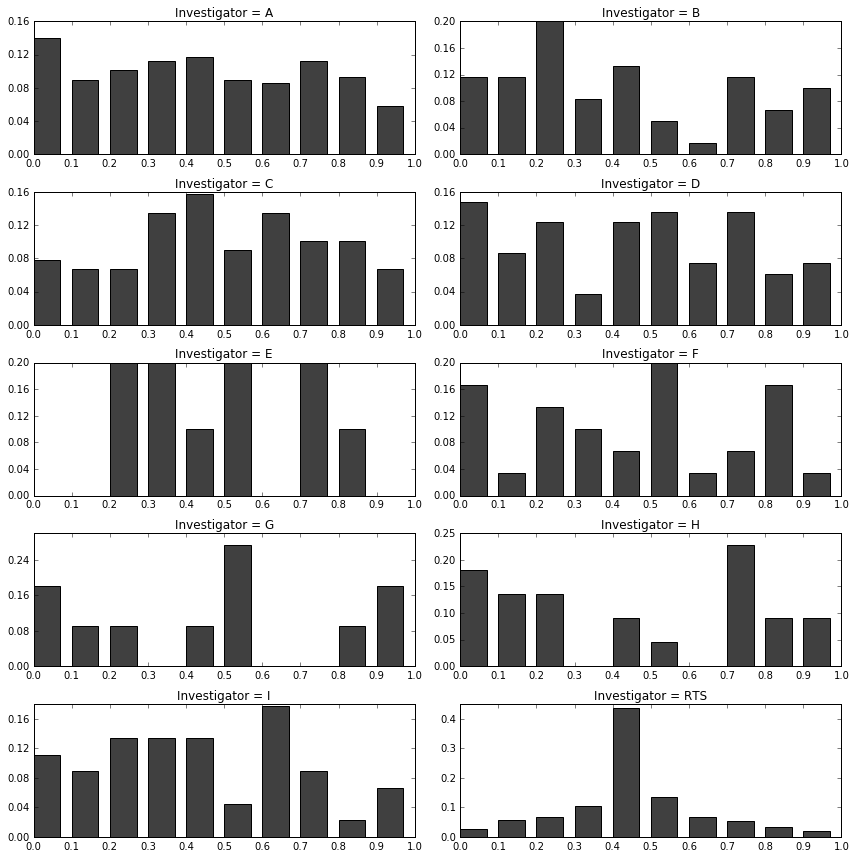
\includegraphics[width=0.8\linewidth]{images/new_mid_ratio.png}
\caption{Individual Histograms for the Colony Data}
\label{ind_mid_ratio}
\end{figure}

Two important observations can be made:
\begin{itemize}
\item
  The histograms for researchers with labels B, C, E, F, G, H, I do not
  appear following uniform distribution.
\item
  RTS heavily influences the histogram when his/her data is collected in the pool and, therefore, patterns from the other researchers look anomalous when compared to it.
\end{itemize}

These points illustrate the limitations of the uniformity assumption for
mid-ratios and the visual comparison between the histograms of RTS and the pool to motivate suspicion. 


    \subsection{Permutation Tests}\label{quick-primer-to-permutation-tests}


``The problem of determining whether a treatment has an effect is widespread in various real world problems. 
To evaluate whether a treatment has an effect, it is crucial to compare the outcome when treatment is applied (the outcome for the treatment group) with the outcome when treatment is withheld (the outcome for the control group), in situations that are as alike as possible but for the treatment. This is called the method of comparison.''\cite{philip}. 
We will describe this method for a specific set up relevant for this review.

Suppose that we are given two sets of observations - one of them labeled as `treatment' with size $T$, and the other labeled as `control', of size $C$. 
We assume that the first of them has received a treatment and we wish to test the hypothesis whether this treatment affects the group. 
In a two-sample permutation test, the data is pooled together
to form a population of size \(N = T+C\).
To compare the two groups, we need to decide on a test-statistic that can capture the effect of the treatment (if any) on the population. 
As an example, we can consider the absolute difference between the sample means of the two datasets.
Under the null hypothesis that the treatment has no effect, one can analytically derive the distribution of this test statistic. 
However, it is often easier to empirically approximate such distribution rather than compute it numerically. 
To do so, one needs to repeatedly randomly  partition the data into groups of size \(T\) and \(C\) and compute the test statistic contrasting the two groups. 
We use the empirical histogram obtained from these experiments, as a proxy for the true distribution of the test statistic. 
Just like typical hypothesis testing, we then determine the chances ($p$-value) of observing the test statistic that we computed in the beginning.

When the $p$-value is below a preset significance level, we infer that the treatment has an effect at that level of significance. It is unlikely that the two sets  were obtained by a random partition of the pooled data.


    \subsubsection{Results for
Mid-Ratio}\label{permutation-tests-for-mid-ratio}

We set the test statistic to be the difference in
standard deviation of the mid-ratios for the two datasets. 
We choose the standard deviation, instead of the mean, because our null and alternative hypothesis for mid-ratio (uniform distribution versus concentration around 0.5) have the same mean ($0.5$). 
We expect the standard deviation to capture
the \textit{unintentional reduction in spread caused in data due to
intentional adjustments}.

We consider each researcher's data equivalent to a treatment group and the rest of them as the control group. 
We use 1000 repetitions to obtain the empirical
distribution and then compute the $p$-values: 
\begin{itemize} 
	\item $0.00$, for investigators A, B,
	D, and RTS;
	\item \(<0.01\), for C, H, I;
	\item  \(>0.01\), for  E,F,G.
\end{itemize}
 The $p$-values indicate that almost all datasets are surprising with respect to this
test-statistic. 
We would like to emphasize that here a $p$-value of $0.00$ in fact denotes a $p$-value $<0.001$, because of the finite resolution owing to $1000$ tests.
We would also like to mention that RTS is still the most surprising if one looks at the location of the test-statistic in the tails of the distribution.

We also use \(\ell_1\)-distance between the density\footnote{abuse of terminology, used in place of normalized histograms}, and the
\(\ell_1\)-distance between the cumulative distribution function (CDF) as the test statistic. Again, we reject several researchers of the lab at a significance level of \(1 \%\). 
We present all the $p$-values in Figure~\ref{mid_ratio_perm}.

\begin{figure}[H]
\centering
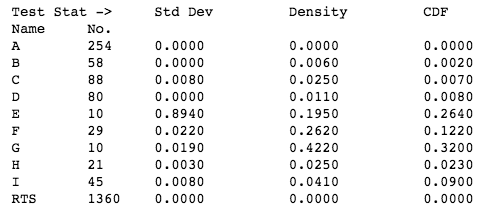
\includegraphics[width=0.8\linewidth]{images/mid_ratio_perm.png}
\caption{Results for Permutation Tests for Mid-Ratio}
\label{mid_ratio_perm}
\end{figure}

{\bf Remark} We would like to mention that when RTS is included in the control group, it constitutes the bulk of the group. As a result, rejecting the null hypothesis for a researcher is almost equivalent to rejecting the hypothesis that the data of that researcher is same as RTS's data. 
If we already believed or discovered that RTS's data was suspicious, then we cannot flag other researchers' data as suspicious. 
Therefore, we do another set of permutation tests after excluding the RTS's data. 
We did not find strong evidence to reject the null hypothesis, hence we conclude that none of the researchers is suspicious at a significance level of $1\%$. 
However, this set of tests suffer from a bias because of our manual throwing away 2/3 of the data points.

\begin{figure}[H]
\centering
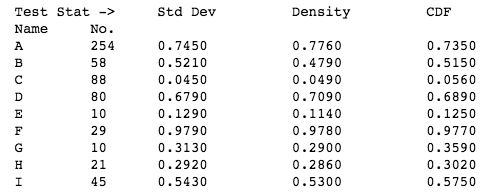
\includegraphics[width=0.8\linewidth]{images/mid_ratio_perm_no_rts.png}
\caption{Results for Permutation Tests without RTS  for Mid Ratios}
\end{figure}

Putting together all the pieces, we conclude that there is statistical evidence to claim that RTS's data is not genuine.

    \subsection{Additional Tests for Digit
Analysis}\label{additional-tests-for-digit-analysis}

For the terminal digit and equal digits analyses, we extended the tests done by
the authors to individual members of the lab and performed (1) chi-square test for goodness of fit for terminal digit, (2) chi-square test for goodness of fit for equal digits and (3) permutation tests for terminal digit. For permutation tests, we used the test statistics listed in the previous section. Results are tabulated in Figures \ref{cst1}, \ref{cst2}, and \ref{perm2}.

\begin{figure}[H]
\centering
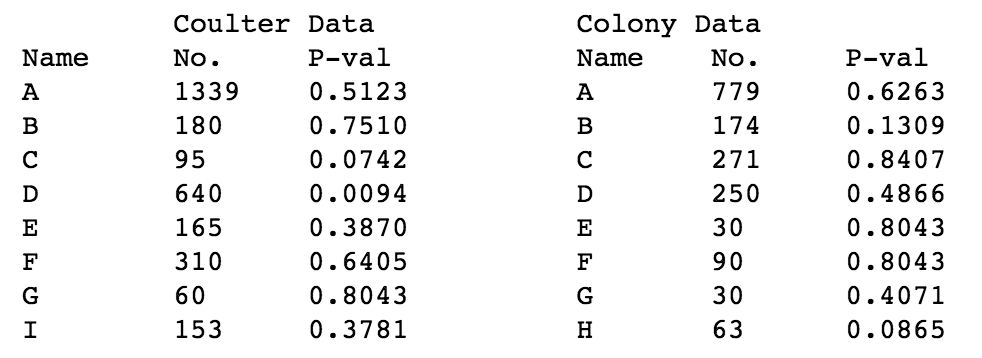
\includegraphics[width=0.7\linewidth]{images/raaz_term_chi_summary.png}
\caption{Chi Square Tests for Terminal Digits in Coulter and Colony
Counts}
\label{cst1}
\end{figure}

\begin{figure}[H]
\centering
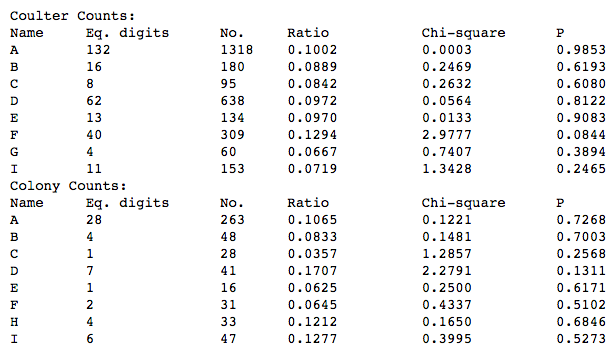
\includegraphics[width=0.9\linewidth]{images/raaz_eq_chi_elaborate.png}
\caption{Chi Square Tests for Equal Terminal Pair in Coulter and Colony
Counts}
\label{cst2}
\end{figure}

\begin{figure}[H]
\centering
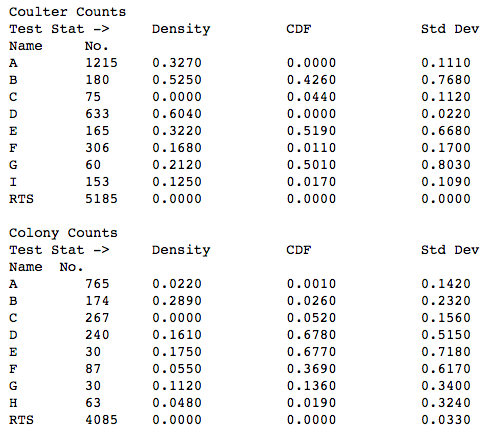
\includegraphics[width=0.7\linewidth]{images/raaz_eq_perm_summary.png}
\caption{Permutation Tests for Terminal Digit Analysis, Coulter Counts}
\label{perm2}
\end{figure}

Figure~\ref{perm2}, once again, confirms that RTS's data is suspicious. As before, the huge fraction of data
by RTS contributes towards the low $p$-values for some of the other
researchers. In permutation tests after excluding RTS, none of the researchers look suspicious. For sake of brevity, we avoid mentioning the
$p$-values here.

    \section{Conclusion}\label{conclusion}

    Data fraud is an extremely critical issue in science, engineering, and
many other fields. Methods to detect manipulated data are needed to
identify fraudulent research behaviors. Detecting frauds, however, is a
delicate matter. Challenging the credibility of a researcher or of a
scientific work, in fact, can have heavy consequences for all the parties
involved in the process. Methodologies and techniques used in this kind
of work need to be clear and widely accepted. They need to produce
results which leave minimal (ideally no) space to ambiguity. Independently, reproducibility of results is a fundamental element to rule out any doubts that could arise at any time.
In our review, we carefully analyzed the authors' work by reproducing the results in the paper and using additional tests which we believe to be more general.
We found that authors' conclusions are correct, having been able to reproduce most of their results. 
Moreover, we encourage the use of more powerful tools, such as permutation tests, which we proved to be effective in the context of the paper. 
Such tests help focusing the analysis not on the assumptions, but on the actual anomalies present in the data.

At the end of our review, we do believe that there is a significant evidence that RTS has suspicious data.
 However, we recommend the authors to collect additional information since some of our tests suggest that other investigator's data have anomalies as well, if we do not discount the huge fraction of data given by RTS.

\section*{Acknowledgments} % (fold)
\label{sec:acknowledgments}

We would like to thank the authors H. Pitt and H. Hill for publishing in an open journal, and making the data available for everyone. Also, we would like to thank Prof Philip Stark for his valuable and critical guidelines and timely feedback. We would also like to thank Yuansi Chen for valuable tips with python. As a final note, we would like to claim complete responsibility for all the opinions expressed in this paper.

% section acknowledgments (end)


\bibliographystyle{apalike}
\bibliography{biblio}

    \end{document}
